\chapter{The $\delta$ Sct stars}
\label{deltascuti}
In this chapter we characterize and describe the $\delta$ Sct stars more in detail, including the stars used in this work. 
\begin{figure}[htbp]
    \centering
    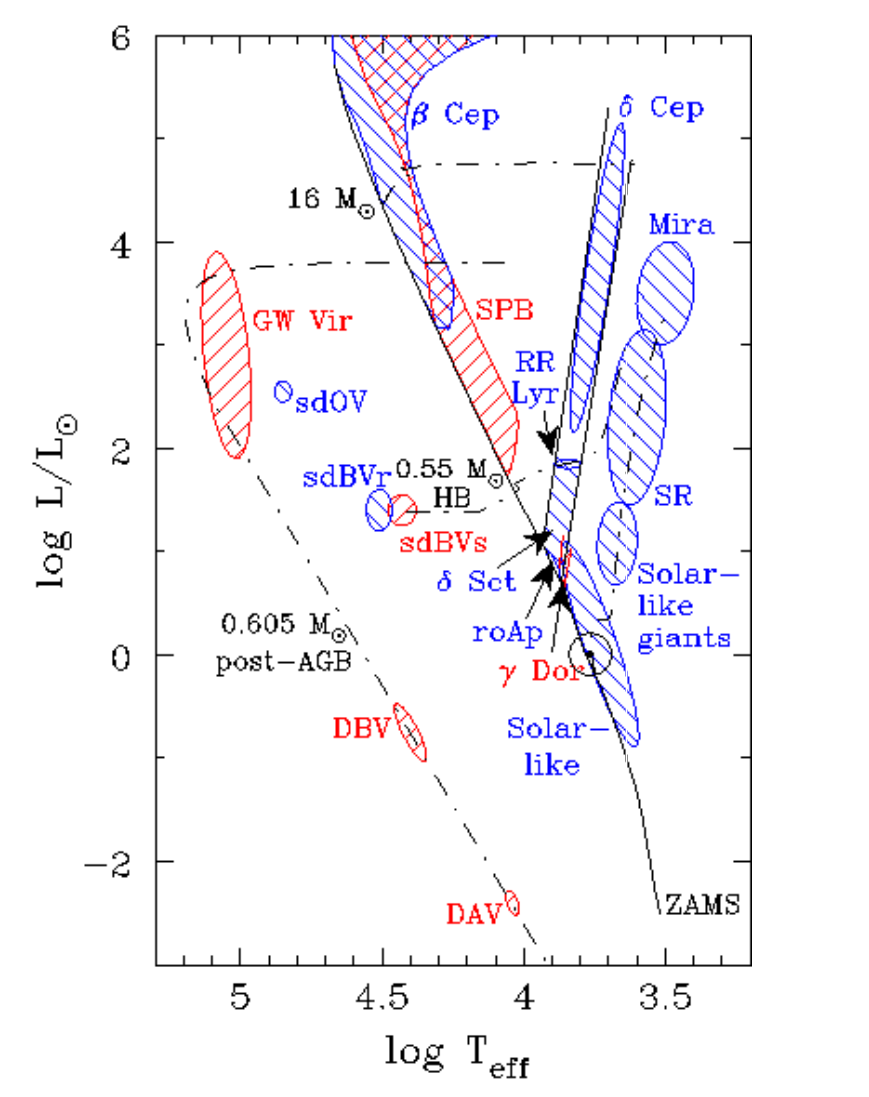
\includegraphics[width=0.9\textwidth]{hrpuls.png}
    \caption{Asteroseismic HRD, showing the different classifications of pulsating stars. }
    \label{hrd}
\end{figure}

\section{The pulsation HR-diagram and the driving mechanisms}
As mentioned in \chapref{chap:asteroseismology}, there are many different types of pulsating stars, situated over the entire Hertzsprung-Russel diagram (HR-diagram). \figref{hrd} illustrates the schematic overview of the various types of stars in the \textit{asteroseismic HR-diagram}. Stars that have p mode pulsations are marked in red, whereas g mode pulsators are blue. The range for which the stars pulsate is marked in the HR-diagram and is called an  \textit{instability strip}(different for each type). The hybrids pulsate in both p and g modes simultaneously and can be found where the instability strips overlap. 

The type of oscillation in a star depends on the \textit{driving mechanism}. For the Sun and solar like-oscillators the primary driving mechanism is the stochastic driving. Acoustic energy from motion in convective cells in the outer convection zone can sufficiently cause a resonance at the star's natural frequencies, where a part of the energy becomes oscillation modes. A mode will be excited in a convection cell and damped when the cell turn over. But since there is a large number of convective cells it will be re-excited immediately after at a different phase. So the excitation is random or \textit{stochastic}. 
For $\delta$ Sct stars, the driving mechanism is different. These are driven by a heat engine, which is a mechanism that transforms thermal energy in a star into mechanical energy of oscillations. When a star contracts the pressure and temperature increases, causing the opacity ($\kappa$) to increase in layers of H and He ionization. This is also why it is called the \textit{$\kappa$-mechanism}. The radiative flux from the core is hence blocked and builds up underneath the layers of higher opacity. The additional stored energy is transformed into mechanical energy, causing the layers to move beyond the equilibrium; the star expands. When the star is heated the H and He atoms will ionize. The ionization of the gas causes a reduction in opacity and radiation can flow through. The gas then cools down so much that it can no longer support the weight of the overlying layers, and the star then contracts recombining H and He. The cycle then repeats itself. 
The zones where the radiative flux becomes trapped are the layers of partial ionization. The first zone is where H and He are ionized around 14.000 K, close to the surface of the star. Second ionization zone is around 40.000 K where He II is partially ionized. Lastly, the innermost zone is where ionization of iron elements occur, at 200.000 K. For $\delta$ Sct stars the driving mechanism excites primarily in the He II ionization layer.   

Yet another type of driving mechanism is the \textit{convective blocking} in Gamma Doradus ($\gamma$ Dor), DA and DB dwarfs. This mechanism is similar to the $\kappa$ mechanism, except the energy is stored in the outer convection zones. Such mechanism gives rise to g-modes oscillations rather than the p-modes from the $\kappa$ mechanism. 

Contrary to the stochastic excitations in solar-like oscillators, the heat engine mechanism does not excite all modes to an observable amplitude, which makes \textit{pattern recognition} challenging.  It is also not well understood why only some modes are excited to an observable amplitude. \citet{dziembowski1990} suggested trapping in the acoustic cavity as an explanation to why only some modes are excited, however could not confirm whether the processs yields a pattern or if it is random. All of these features makes it difficult to determine the frequency of the mode i.e. \textit{mode identification}. For stochastic oscillations, we are able to derive relations to estimate stellar age \citep{kjeldsen2011amplitudes}, however such relations has not yet been found for $\delta $ Sct stars. Therefore, mode identification is significantly more empirical and must be assessed with a  more practical approach rather than theoretical.  

%remember to mention turbulent pressure

\section{Why $\delta$ Sct stars?}
\label{sec:why}

The main focus of this thesis is the $\delta$ Sct stars. In the pulsating HR-diagram $\delta$ Sct pulsators are located in the lower part of \textit{the classical instability strip}. As mentioned previously they pulsate due to the $\kappa$ mechanism acting in the He II ionization zone. In the HRD, the region of $\delta$  Sct  pulsations is marked is defined by the $red edge$ and $blue edge$. The location of these edges is defined by the effective temperature of the $\delta$ Sct star. Higher effective temperature means that the opacity bump will be located deeper in the star where the star is denser. Therefore, the blue edge indicates the maximum effective temperature for which the He II opacity bump is still located at densities where the $\kappa$ mechanism can excite pulsations \citep{pamyatnykh2000}. At temperatures lower than the red edge the convective layers go deep enough that oscillations are damped. These boundaries were calculated theoretically by considering the interaction between pulsation and convection \citep{grigahcene2005convection, dupret2004theoretical}.  

The $\delta$ Sct stars have spectral types from A0 to F2, with pulsation periods between 18 minutes and 8 hours. They can be found on the PMS, MS and immediate post-MS, and their masses range from around 1.5 to 2.5 solar masses. There are several types of $\delta$ Sct pulsators, but historically they are divided into two main groups: High-amplitude $\delta$ Sct pulsators (HADS) with amplitudes of the dominant modes around 0.3 mag. Radial pulsations are dominant for these types. A vast majority of these types have low projected rotational velocities, which is good for modeling purposes as discussed in \chapref{sec:asteroseismology}. The second group is the low-amplitude $\delta$ Sct pulsators (LADS) which pulsate in many non-radial modes and are suggested to have higher projected rotational velocities with an average $v\sin i$ of 96 $km s^{-1}$ \citep{solano1997spectroscopic}.

There are several reasons why these intermediate mass stars are of particular interest for understanding stellar evolution. They occupy a region in th HRD where many processes occur. They are at the transition where the outer convection layer goes from deep and active to shallow an ineffective. Additionally, stars in the classical instability strip have a convective core, which gives rise to convective processes near the core that cannot be found in the Sun. The reason this transition is so important is not only because it has an impact on the stability of pulsation but also on the mixing processes, evolution and particularly the lifetime. Therefore, understanding these processes in these stars makes it possible to project that knowledge to stellar evolution in general. The $\delta$ Sct stars also have the advantage that the p modes probes the layers where these processes occur. Stars that follow the following criteria are better subjects for studying. 

\begin{itemize}
    \item Every single additional pulsation frequency contain valuable information about the star. Therefore it is desirable to have a wide range of both radial and non-radial modes. 
    \item As discussed in \chapref{chap:asteroseismology}, rotation causes numerous effects that cannot be ignored in mode identification (rotational splitting) and modeling. Therefore,  $\delta$ Sct stars with low rotational velocities are favored. 
\end{itemize}

For these reasons 44 tau is a good candidate for studying and modeling. The results and methods can then be applied to stars where mode id has been less successful and modeling is needed. In this study, this will be HD 187547 \citep{antoci2014role}. 

\section{The delta Scuti stars 44 Tau and HD 187547}

\subsection{44 Tau}

44 tau is a class F2 IV $\delta$ Sct star. The observational background and history of 44 Tau will be briefly presented here. For more details on the full observational history, see \citet{antoci200744}. Photometric campaigns were conducted by the \textit{Delta Scuti Network} from 2000-2003. Here, an extensive frequency analysis was performed, and the rotational velocity has been determined to be as low as $2 \pm 1 km s^{-1}$ \citep{lenz2008asteroseismic}. Since the average projected rotational velocity of early F-type stars is $114 \pm 5 km s^{-1}$ \citep{royer2004rotational}, this is a very small value, which lead to the discussion if the star is a slow rotator or if it is observed pole-on\citep{antoci200744}. 
 %The projected rotational velocity has been determined to be as low as 2 km$ \pm 1 s^{-1}$ \citep{lenz2008asteroseismic}
 An additional multisite campaign  was initialized in 2004 \citep{zima2007high} and \citet{breger2008A&A} contributed with frequency analysis from seasons  2004/5 and 2005/6, giving a total of 6 years of photometry data. This yielded a total of 49 frequencies. These frequencies presented in \tabref{freqs}. \citet{zima2007high} confirmed that 44 Tau is an intrinsically slow rotator by constraining the inclination angle to $60 \pm 25^{\circ}$ with an equatorial rotation rate of $3 \pm 2 km s^{-1}$. Atmospheric parameters were derived from spectroscopy to be  $T_{eff} = 7000\pm200 K$ and $\log g = 3.6\pm0.1$ \citep{zima2007high}.

 %A revision of the initial Strömgren indices lead to the determination of an effective temperature of $T_{eff} = 7000 \pm 200$ and \logg value of $3.7\pm 0.1$. 
\begin{table}[htbp]
	\centering
	\caption{Observed frequencies of 44 Tau with the corresponding mode identification \citep{lenz2010delta}. }
	\label{freqs}
\begin{tabular}{lll}
\toprule
         & Frequency [$d^{-1}$]  & $(l,m)$ \\ \midrule
$f_1$  & 6.898 $ \pm 7.43 \cdot 10^{-7}$ & (0,0)    \\
$f_2$  & 7.006 $ \pm 2.01 \cdot 10^{-6}$ & (1,1)    \\
$f_3$  & 9.117   $ \pm 2.36 \cdot10^{-6}$ & (1,1)     \\
$f_4$  & 11.52   $ \pm 1.10 \cdot 10^{-6}$ &  (1,0) \\
$f_5$  & 8.960  $ \pm 2.24 \cdot 10^{-6}$ & (0,0)     \\
$f_6$  & 9.561   $ \pm  3.09\cdot 10^{-6}$ &  (1,-)  \\
$f_7$  & 7.303  $ \pm  4.62 \cdot 10^{-6}$ &  (2,0) \\
$f_8$  & 6.795  $ \pm  8.97 \cdot 10^{-6}$  &  (2,0)    \\
$f_9$  & 9.583 $ \pm 1.71\cdot 10^{-5}$ &  (2,-)   \\
$f_{10}$ & 6.339  $ \pm 1.40 \cdot 10^{-5} $& (2,-)    \\
$f_{11}$ & 8.639  $ \pm  1.33\cdot  10^{-5}$ &  (-,0)   \\
$f_{12}$ & 11.29 $ \pm     2.17\cdot 10^{-5} $ &    \\
             
\end{tabular}
\end{table}

%For a full asteroseismic analysis, knowledge on the stellar parameters is needed. These can be derived from the results of Strömgren and Geneva photometry. The Strömgren indices of uvby$\beta$ \citep{hauck1997vizier} are shown in \tabref{stromgren}.

%\begin{table}[htbp]
%\begin{tabular}{lllll}
%\hline
%V {[}mag{]}       & b-y {[}mag{]}     & $m_1$ {[}mag{]}   & $c_1$ {[}mag{]}    & $\beta$           \\ \hline
%5.390 $\pm$ 0.040 & 0.215 $\pm$ 0.005 & 0.170 $\pm$ 0.005 & 0.755 $\pm$  0.009 & 2.711 $\pm$ 0.006 \\ \hline
%\end{tabular}
%\caption{Measured Strömgren indices for 44 Tau}
%\label{stromgren}
%\end{table}

No significant interstellar reddening has been found, and the metallicity was determined to be close to that of the sun by \citet{mcnamara1985relations}. From this metallicity the Vienna NEMO grid (Model Grid of Stellar Atmospheres, \citet{nendwich2004interpolation}, \citet{heiter2002new}) can be employed to derive an effective temperature and surface gravity. This was done by \citet{lenz2008asteroseismic}, yielding $ \log T_{eff}= 3.839 \pm 0.007$ ($T_{eff} = 6900 \pm 100 K$), in agreement with the spectroscopic value. Based on the HIPPARCOS parallax of $16.72\pm 0.93 mas$ a luminosity of $\log L/\L_\odot = 1.340 \pm 0.065$ was also derived. This was revised with a new bolometric correction to $\log L/L_\odot = 1.305 \pm 0.065$ \citep{lenz2010delta}. 

The recent data release for the GAIA mission has provided new atmospheric parameters for both 44 Tau and HD 187547. GAIA data release 2 was released on 25 April 2018 and is available through the Gaia Archive \citep{brown2018gaia}. GAIA conducts three-band photometry on bright sources, assuming that they are single stars. From the three-band photometry, measured parallax and training sets, estimates on \teff and $R$ are made. 
The luminosity can be derived through the G-band magnitude $M_G$ and bolometric correction $BC_G$:

\begin{equation}
	-2.5\log L = M_G + BC_G(T_{eff}) - M_{bol,\odot}, \quad M_{bol,\odot}
\end{equation}

Some systematic errors were detected by \citet{andrae2018gaia}. The GAIA atmospheric parameters for 44 Tau is listed along with the HIPPARCOS and spectroscopic values in \tabref{obsparams}. 

\begin{table}[htbp]
	\caption{Observational parameters listed as given by \citet{lenz2010delta} and \citet{brown2018gaia}. The "parameter set column" divides the observational parameters into to consecutive runs done for 44 Tau.}
	\label{obsparams}
\centering
\begin{tabular}{|l|lll|}
\hline
                                                   & Value                                             & Reference  & Parameter set\\ \hline
$\log g $                                  &  $3.6 \pm 0.01$                            & \citep{zima2007high} & 1 and 2   \\
$\log T_\text{eff}$             & $3.839  \pm 0.007$                   &   \citep{lenz2010delta}  & 1 \\
$\log T_\text{eff, GAIA}$ &  $3.843^{+0.003}_{-0.007}$ & \citep{brown2018gaia} & 2\\
$\log (L/L_\odot)_{HIP}$                  &  $1.305 \pm 0.065$                          & \citep{lenz2010delta}  & 1   \\
$\log (L/L_\odot)_{GAIA}$& $1.383 \pm 0.004$                        &  \citep{brown2018gaia}  & 2 \\ \hline
\end{tabular}
\end{table}

During this project, two difference runs will be made to implement the values for different parameters sets. Firstly, a run will be made with the \citet{lenz2010delta} photometric \teff and \lum with the spectroscopic \logg. Second run will be made with the GAIA \teff and \lum (\logg will be the same). In order to verify the GAIA values of \lum a calculation was made based on the GAIA parallax, bolometric correction from \citet{Flower96} and B and V magnitudes from the Tycho-2 catalogue. This yielded a value of $\log (L/L_\odot)_{gaia} = 1.3572 \pm 0.0082$. This value will not be further investigated in the runs, but is made for making the point that parameters from GAIA (or any other mission) should not be used without considering their reliability and updates. 



%%The luminosity can be derived from the parallax, either from Hipparcos ($\log L_{hip} = 1.305 \pm 0.065$, $p = 16.72 \pm 0.93$ mas) or Gaia  ($\log L_{Gaia}$, $p=15.3323 \pm 0.1307$ mas) from GAIA's data release 2 catalog \citep{clementini2017gaia, brown2018gaia}. Whereas $\log L_{Gaia}$ was derived by \citet{lenz2010delta}, the Gaia luminosity is instead calculated using 
%
%\begin{equation}
%    m_{bol} = M_{bol} + 5\log(d) - 5, \quad m_{bol} = V + BC, \quad M_{bol}- M_{bol,\odot} = -2.5\log\left(\frac{L}{L_\odot}\right),
%\end{equation}
%
%\noindent yielding
%
%\begin{equation}
%    \log\left(\frac{L}{L_\odot}\right) = \frac{V + BC - 5 \log(d) + 5-M_{bol,\odot}}{-2.5}, \qquad d = \frac{1\text{pc}}{p\;\text{arcsec}}.
%\end{equation}
%
%\noindent where $M_{bol,\odot} = 4.74$ and the bolometric correction is set to $BC = 0.032$ using tables from \citep{Flower96} and $V=5.387 \pm 0.009$ \citet{hog2000tycho}. Inserting these values gives a luminosity of $log L_{gaia} = 1.3572 \pm 0.0082$. Uncertainties are calculated by
%
%\begin{equation}
%    \sigma_{\log L}^2 = \left(\frac{\partial L}{\partial V}\right)^2 \sigma_V^2 + \left(\frac{\partial L}{\partial p}\right)^2 \sigma_p^2 + \left(\frac{\partial L}{\partial BC}\right)^2 \sigma_BC^2,
%\end{equation}

%\noindent where $\sigma_{BC}$ is set to 0.001 (based on three decimals on the numbers in \citet{Flower96}. 


Mode identification yielded a confident identification of the radial fundamental mode and the first overtone \citep{lenz2008asteroseismic}. Constraining models with these two frequencies has a major advantage in modeling, and \citet{lenz2010delta} successfully reproduced the observed frequency range using stellar evolution models from the Warsaw new Jersey code developed by combined with a stellar pulsation code \citep{paczynski1969envelopes}. The best model showed that 44 Tau is on the post-MS and more specifically in the contraction phase. Relative to the time spent on the MS for these stars, the lifetime in this phase is extremely short and therefore difficult to resolve in the HRD. Hence, modeling is of great importance when studying the evolutionary stage of a star. 
\\


\subsection{HD 187547}

Like 44 Tau, HD 187547 is a $\delta$ Sct star. It was observed  with the NASA spacecraft \textit{Kepler} \citep{koch2010kepler}. The first observations were taken over thirty days with one minute cadence. The frequency spectrum on \figref{ssspectrum} shows a large range of pressure modes for both high and low order radial modes, which could not be explained solely by the $\kappa$ mechanism. The frequency range is from $45-80 d^{-1}$. Follow up ground-based observations were conducted during 2010 \citep{antoci2011excitation}, mainly spectroscopy; see \citet{antoci2011excitation} supplementary material for more information. Initially, \citet{antoci2011excitation} interpreted the high radial overtones as being stochastically excited, and thereby reported HD 187547 as the first $\delta$ Sct star where solar-like oscillations predicted by \citet{houdek1999, samadi2002} were detected.  However, an analysis carried out on an additional 960 days short cadence observations revealed that the spectrum is not consistent with a coherent signal (\figref{ss2}), but is suggested to be related to turbulent pressure \citep{antoci2014role}. 

\begin{figure}[htbp]
    \centering
    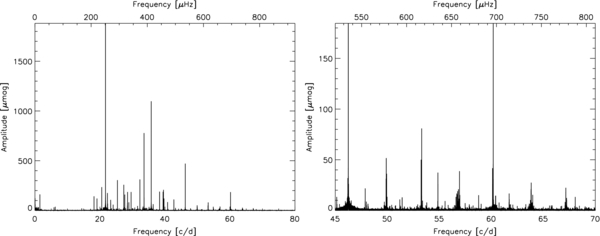
\includegraphics[width=1\textwidth]{superstarspectrum.jpg}
    \caption{Fourier spectra of the Kepler short cadence data. Right panel: close-up in the frequency region interpreted by \citet{antoci2011solar} to be stochastically excited. Figure and caption from \citet{antoci2014role}}
    \label{ssspectrum}
\end{figure}

\begin{figure}[htbp]
    \centering
    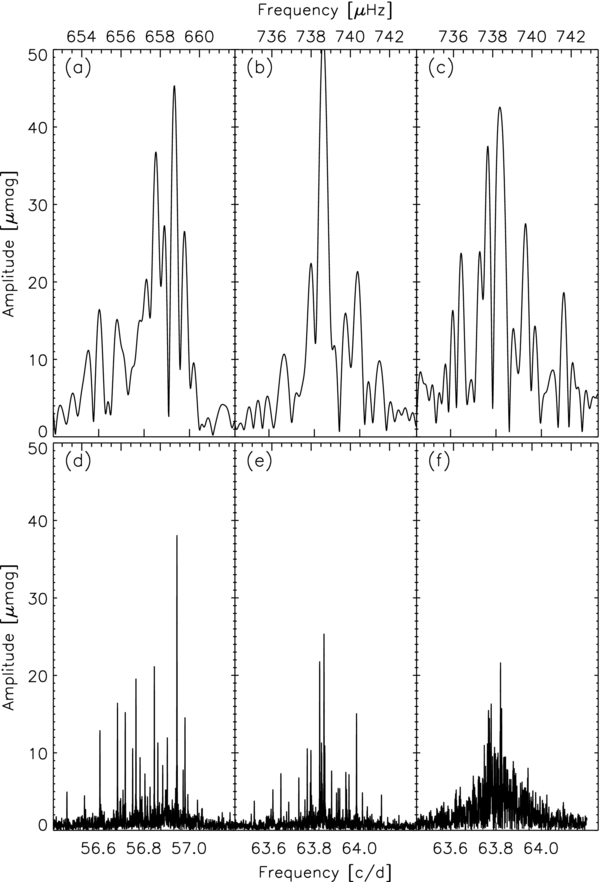
\includegraphics[width=0.8\textwidth]{superstar2.jpg}
    \caption{In panels (a), (b), (d), and (e), the Fourier spectra of two different oscillation modes observed in HD 187547 is shown. Panels (c) and (f) show simulated stochastic, damped, and re-excited oscillation mode. The Fourier spectra in panels (a), (b), and (c) are based on 30 days of observations (quarter 3.2,\citep{antoci2011solar}). Panels (d) and (e) illustrate the oscillation spectra of HD 187547 based on 960 days of short-cadence data. It can be seen that for a stochastic signal the amplitude decreases with increasing observing time, which does not occur in coherent modes. Figure and caption from \citet{antoci2014role}}
    \label{ss2}
\end{figure}

The spectroscopic observations made by \citet{antoci2011excitation} led to estimates on the atmospheric parameters $T_{eff} = 7500 \pm 250$, surface gravity of $\log g = 3.90 \pm 0.25$ and a projected rotational velocity of $v \sin_i = 10.3 \pm 2.3 kms^{-1}$. A photospheric metallicity of Z = 0.017 was also derived by \citet{antoci2011excitation}. The analysis of the high-frequency modes lead to the determination of a large frequency separation of $\Delta \nu = 3.5 \pm 0.05 d^{-1}$. Models with $\log L/L_\odot \approx 1.3$ were used for the purpose of modeling the star. However, observations from GAIA has provided new reviewed parameters with a significantly lower $ \log L/L_\odot = 0.859 \pm 0.003$. The luminosity was also derived by the same method as for 44 Tau in this project, leading to a value of $\log L/L_\odot \approx 0.837$. The low value of the luminosity could indicate that the star is not as far in its evolution as \citet{antoci2011excitation, antoci2014role} anticipated. This would also mean that the $\Delta \nu $ value should be reviewed, even doubled to $\Delta \nu = 7 d^{-1}$ (Private communication with Victoria Antoci, Tim Bedding et al. in review). The main focus for HD 187547 will therefore be to determine what $\Delta \nu$ is best reproducing the observed parameters. 


\begin{table}[htbp]
	\centering
	\begin{tabular}{|l|ll|}
		\hline
		& Value                                             & Reference \\ \hline
		$\log g$                                  &  $3.9 \pm 0.02$                            & \citep{antoci2011excitation}    \\
		$\log T_\text{eff}$             & $3.875  \pm 0.0011$                   &   \citep{antoci2011excitation}   \\
		$\log T_\text{eff, GAIA}$ &  $3.900 \pm 0.002$                  & \citep{brown2018gaia} \\
		$\log (L/L_\odot)_{GAIA}$& $0.859 \pm 0.003\footnotemark{}$                   &  \citep{brown2018gaia}   \\ \hline
	\end{tabular}
\end{table}

\footnotetext{The values from GAIA have not considered reddening which is relevant for HD 187547. Therefore they should be used with care.}

Besides the peculiar frequency spectrum, an analysis of the abundances of HD 187547 classified it as a chemically peculiar Am star. This means that it shows photospheric overabundances in Ba, Y, and Sr and underabundances in Sc and Ca \citep{preston1974chemically}. Particularly of interest are the pulsating AmFM stars, since they do not comply well with predictions from the $\kappa$-mechanism. The theory states that settling of He causes an underabundance in the He II ionization layer, hence the $\kappa$-mechanism cannot drive the pulsation sufficiently. \citet{turcotte2000} implemented diffusion of heavy elements into the models to account for only a very tightly constrained instability region. However AmFm are not only observed in this region, but over the entire $\delta$ Sct instability strip \citep{smalley2011superwasp, balona2011kepler}. In that sense, HD 187547 is interesting not only because of its wide frequency range, but also because those frequencies are even more unusual for a pulsating Am star. Therefore it is of great interest to model this star to gain information on the nature of the pulsations. 
\\

%Mode identification has not yet provided any reliable results, and further analysis is needed to give information on the nature of the frequencies, and particularly constrain models of the star. 

